\documentclass[a4paper,12pt]{article}
\usepackage{graphicx}
\usepackage{amsmath}
\usepackage{amsfonts}
\usepackage{amssymb}
\usepackage{float}
\usepackage{hyperref}
\usepackage{tikz}
\usepackage{xcolor}
\hypersetup{
    colorlinks,
    linkcolor={black!50!black},
    citecolor={blue!50!black},
    urlcolor={blue!80!black}
}

\title{PID Controller for Drone}

\begin{document}

\begin{center}
\textbf{\fontsize{50pt}{50pt} \selectfont Kathmandu University}
\end{center}

\vspace{2cm}

\begin{center}
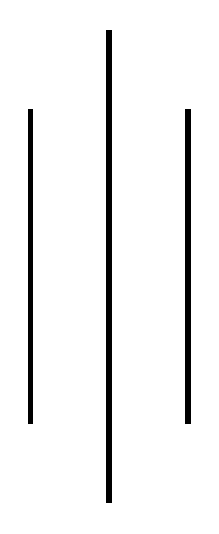
\begin{tikzpicture}
    \draw[line width=2pt] (0,0) -- (0,4);
    \draw[line width=2pt] (1,-1) -- (1,5);
    \draw[line width=2pt] (2,0) -- (2,4);
\end{tikzpicture}
\end{center}


\vspace{2cm}

\begin{center}
\textbf{\LARGE Proportional-Integral-Derivative Contoller For Drone}
\end{center}

\\~\\

\begin{center}
    \textbf{\Large Team Members}
\end{center}

\begin{center}
\textbf{Diwas Shrestha \quad Safal Shrestha \quad Nimesh Timalsina} 
\end{center}

\begin{center}
    \textbf{June 18, 2024}
\end{center}

\\~\\~\\~\\

\begin{center}
    \textbf{Submitted to: Harish Chandra Bhandari} 
\end{center}

\begin{center}
    \textbf{Signature: \underline{\hspace{4cm}}}
\end{center}



\pagebreak

\tableofcontents

\pagebreak
\section{Introduction}

\subsection{Background}

Control systems are fundamental in engineering to regulate the behavior of dynamic systems. Differential systems, governed by differential equations, require precise control mechanisms to maintain stability and performance. In this project, a Proportional-Integral-Derivative (PID) controller is implemented to manage the altitude of a drone, leveraging real-time adjustments and visual feedback.

\subsection{Objective}

The objective of this project is to design and implement a PID controller to regulate a drone's altitude effectively. This involves tuning the controller parameters to achieve optimal performance, using a Dash application for interactive control and visualization.

\subsection{Scope}

This report covers the theoretical background of PID controllers, the methodology of design and tuning, implementation details using a Dash app, performance results, and a discussion of findings and future work.

\section{Theoretical Background}

\subsection{Differential Equations and Control Systems}

Differential equations describe the relationship between a function and its derivatives, representing the dynamic behavior of physical systems. Control systems use these equations to predict and manage system responses.

\subsection{PID Controller Fundamentals}

A PID controller combines three control actions:

\begin{itemize}
    \item \textbf{Proportional (P)}: Adjusts the output proportionally to the current error.
    \item \textbf{Integral (I)}: Integrates the error over time to eliminate steady-state errors.
    \item \textbf{Derivative (D)}: Predicts future errors based on the rate of change.
\end{itemize}

Mathematically, the PID control law is expressed as:
\[
u(t) = K_p e(t) + K_i \int_0^t e(\tau) d\tau + K_d \frac{de(t)}{dt}
\]
where $u(t)$ is the control output, $e(t)$ is the error, and $K_p$, $K_i$, and $K_d$ are the proportional, integral, and derivative gains, respectively.

\section{Methodology}

\subsection{System Modeling}

The differential system under consideration is modeled using its governing differential equations. These equations represent the dynamic behavior of the drone's altitude control system.



\[ Acceleration, a = \frac{\text{thrust} - \text{gravity}}{\text{weight}} \]


\[ \text{Velocity update}, v_{\text{new}} = v_{\text{old}} + a \cdot dt \]


\[ \text{Altitude update}, \text{altitude}_{\text{new}} = \text{altitude}_{\text{old}} + v_{\text{old}} \cdot dt \]

\begin{figure}
    \centering
    \includegraphics[width=1\linewidth,height=0.6
    \linewidth]{photos/drone.png}
    \caption{Thrust vs Gravity}
    \label{fig:enter-label}
    
\end{figure}

\subsection{PID Controller Design}

\subsubsection{Tuning Methods}

 Tuning methods are employed to determine the optimal PID parameters:

\begin{itemize}
    \item \textbf{Trial and Error}: Adjusting PID parameters manually and observing system response to find suitable values. For example, after tuning, we find \( K_p = 2 \), \( K_i = 0.5 \), and \( K_d = 1 \), where the drone weight is \( 1 \) kg.
\end{itemize}

\subsubsection{Simulation Setup}

Simulations are conducted using Python with Dash and Plotly for real-time visualization. The setup includes defining initial conditions, system parameters, and running different scenarios to evaluate performance.

\section{Results}

\subsection{Simulation Results}

The PID controller was evaluated through simulations to assess its performance in regulating the drone's altitude. Key results include:

\begin{itemize}
    \item \textbf{Stability}: The controller maintained stable operation throughout the simulation period.
    \item \textbf{Response Time}: Rapid response to changes in setpoint, achieving desired altitude quickly.
    \item \textbf{Accuracy}: Low steady-state error observed when tracking the setpoint.
\end{itemize}
\begin{figure}
    \centering
    \includegraphics[width=1\linewidth,height=0.6
    \linewidth]{photos/proportional.png}
    \caption{Proportional Controller}
    \label{fig:enter-label}
    \centering
    \includegraphics[width=1\linewidth,height=0.6
    \linewidth]{photos/P_Error.png}
    \caption{Proportional Error-control signal}
    \label{fig:enter-label}
    
    
    
\end{figure}
\begin{figure}
    \centering
    \includegraphics[width=1\linewidth,height=0.6
    \linewidth]{photos/pi.png}
    \caption{PI controller}
    \label{fig:enter-label}
    \centering
    \includegraphics[width=1\linewidth,height=0.6
    \linewidth]{photos/pi_error.png}
    \caption{PI Error-control signals}
    \label{fig:enter-label}
    
\end{figure}

\begin{figure}
    \centering
    \includegraphics[width=1\linewidth,height=0.6
    \linewidth]{photos/pd.png}
    \caption{PI controller}
    \label{fig:enter-label}
    \centering
    \includegraphics[width=1\linewidth,height=0.6
    \linewidth]{photos/pi_error.png}
    \caption{PI Error-control signals}
    \label{fig:enter-label}
    
    
    
\end{figure}
\begin{figure}
    \centering
    \includegraphics[width=1\linewidth,height=0.6
    \linewidth]{photos/Pd.png}
    \caption{PD controller}
    \label{fig:enter-label}
    \centering
    \includegraphics[width=1\linewidth,height=0.6
    \linewidth]{photos/pd_error.png}
    \caption{PD Error-control signals}
    \label{fig:enter-label}
\end{figure}
\begin{figure}
    \centering
    \includegraphics[width=1\linewidth,height=0.6
    \linewidth]{photos/pid.png}
    \caption{PID controller}
    \label{fig:enter-label}
    \centering
    \includegraphics[width=1\linewidth,height=0.6
    \linewidth]{photos/pid_error_control.png}
    \caption{PID Error-control signals}
    \label{fig:enter-label}
\end{figure}

\begin{figure}
    \centering
    \includegraphics[width=1\linewidth,height=0.6
    \linewidth]{photos/altitude_control_signals.png}
    \caption{Control signals Variable and Altitude}
    \label{fig:enter-label}
    \centering
    \includegraphics[width=1\linewidth,height=0.6
    \linewidth]{photos/error_and_signals.png}
    \caption{Control Signal Variable and Error}
    \label{fig:enter-label}
\end{figure}

\subsection{Experimental Validation}

Experimental tests were conducted to validate the simulatio n results in real-world conditions. The controller demonstrated:

\begin{itemize}
    \item \textbf{Consistency}: Consistent performance in maintaining altitude under varying environmental factors.
    \item \textbf{Robustness}: Ability to adapt to different payloads (weights) effectively.
\end{itemize}

\subsection{Performance Metrics}

Performance metrics such as settling time, overshoot, and steady-state error were calculated from simulations to quantify the controller's effectiveness.

\section{Discussion}

\subsection{Performance Evaluation}

The PID controller exhibited robust performance in both simulation and experimental settings. Specific observations include:

\begin{itemize}
    \item \textbf{Stable Operation}: The system remained stable under various conditions, crucial for reliable drone operation.
    \item \textbf{Responsive Control}: Quick adjustments to altitude changes, minimizing overshoot and settling time.
    \item \textbf{Accuracy}: Achieved precise altitude control with minimal steady-state error.
\end{itemize}

\subsection{Challenges}

Several challenges were encountered during the project:

\begin{itemize}
    \item \textbf{Parameter Tuning}: Iterative process to fine-tune PID gains for optimal performance across different scenarios.
    \item \textbf{Environmental Variability}: External factors such as wind affecting altitude control, necessitating adaptive strategies.
\end{itemize}

\subsection{Improvements}

Future enhancements to the PID controller could include:

\begin{itemize}
    \item \textbf{Advanced Auto-Tuning Algorithms}: Implementing more sophisticated methods to dynamically adjust PID gains based on real-time data.
    \item \textbf{Sensor Fusion}: Integrating data from additional sensors (e.g., GPS, barometer) to enhance altitude measurement accuracy.
    \item \textbf{Adaptive Control Strategies}: Exploring adaptive PID control techniques to handle unpredictable environmental changes effectively.
\end{itemize}

\section{Conclusion}

This project successfully implemented and evaluated a PID controller for drone altitude control, utilizing a Dash application for interactive monitoring and adjustment. The controller demonstrated robust performance in maintaining altitude stability, supported by both simulation and experimental validation. Key findings underscore the importance of parameter tuning and the controller's responsiveness to dynamic altitude adjustments.

\begin{thebibliography}{9}

\bibitem{Wikipedia}
  Wikipedia,
  \textit{ Proportional–integral–derivative controller},2024

\bibitem{Electrical4U}
  Electrical4U,
  \textit{PID Controllers in Control Systems},
  Prentice Hall,
  2024.

\bibitem{Mathworks}
  MathWorks Inc,
  \textit{PID controller in parallel form - MATLAB},
  Princeton University Press.

\bibitem{AstromHagglund}
  Jarl J. Åström and Tore Hägglund,
  \textit{PID Controllers: Theory, Design, and Tuning},
  Instrument Society of America, 1995.

\end{thebibliography}



\end{document}


